\documentclass[a4paper, 12pt]{report}
\usepackage[italian]{babel}
\usepackage{graphicx}

\begin{document}
\title{

\includegraphics[scale=1]{Immagini/logounipi.png} \\
\vspace*{1in}
\textbf{Descrizione Interfacce}}
\author{Dario Ayrton Corveddu\\
        Federico Giannotti\\
        Francesco Nicolò\\
        Stefano Piccoli\\
		\vspace*{0.5in} \\
		Laboratorio di basi di dati 2021-2022\\
        Prof: Giovanna Rosone
       } \date{\today}
\maketitle
\tableofcontents
	\chapter*{Introduzione}
	\addcontentsline{toc}{chapter}{Introduzione}
        \paragraph{}Il documento di Descrizione delle Interfacce ha l'obiettivo di definire gli standard da utilizzare allo 
        scopo di rendere omogenei la documentazione e il codice prodotti nelle successive fasi.
        Il pacchetto ModGUI offre un insieme di procedure in PL/SQL che determinano lo stile e il comportamento
        delle componenti che interagiscono principalmente con gli utenti. Gli elementi, quindi, una volta forniti dei 
        parametri necessari, andranno a comporre la pagina Web finale.

    \chapter{Progettazione delle operazioni}
        \section{Diagramma degli stati}
            \paragraph{}Per descrivere le operazioni utilizzeremo il \textbf{diagramma degli stati}.\\
            Il diagramma degli stati è un grafo orientato composto da archi e nodi dove i nodi rappresentano gli stati
            e gli archi le transizioni, che sono provocate da vari eventi, etichettati da un nome e dai relativi parametri.
            Distinguiamo due tipi di stati:
            \begin{itemize}
                \item \textbf{Interfaccia:} È lo stato che permette interazione utente-sistema.
                \item \textbf{Processo:} È lo stato composto da un insieme di operazioni sequenziali che elaborano dati.
            \end{itemize}  
            \begin{figure}[htbt]
                \centering
                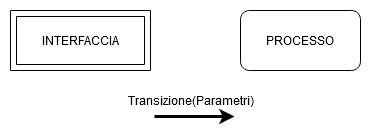
\includegraphics[scale=0.8]{Immagini/elementiDiagrammi.png}
                \caption{Tipi di diagrammi degli stati}
            \end{figure}
        \clearpage
        \section{Convenzioni}
            \paragraph{}Si elenca una lista di convenzioni da adottare nella fase di progettazione:
            \begin{enumerate}
                \item Tutte le pagine devono essere raggiungibili a partire dalla Home oppure da altre pagine.
                \item Non può essere permesso ad un utente che non ha effettuato il login di visualizzare pagine all'infuori della pagina HOME.
                \item È consigliato prevedere uno stato di conferma nelle operazioni cruciali come le eliminazioni definitive.
                \item Un utente, in ogni fase di compilazione di dati, deve avere la possibilità di annullare la procedura tramite un apposito bottone.
                \item Ogni pagina deve essere intitolata in relazione al nome della relativa procedura.
                \item Ogni operazione che prevede immissione di dati da parte dell'utente dovrà prevedere uno stato intermedio di controllo dei dati immessi e, successivamente, una notifica a schermo del risultato, con esito positivo o negativo, dell'operazione.
                \item Ogni pagina di esito deve permettere il raggiungimento della pagina principale senza l'utilizzo dei navigatori del browser.
                \item È possibile prevedere un bottone che permette il ritorno ad una pagina precedente o principale, ma rispettando l'integrità del database.
                \item Ogni interfaccia che ha come scopo l'immissione dei dati da parte dell'utente deve prevedere un bottone ben visibile di invio dati con la funzione submit.
                \item È consigliato inserire nei form di immissione dati un bottone che permette il ripristino ai valori di default dei dati.
                \item Le pagine di visualizzazione devono contenere una modalità di filtraggio dati per velocizzare la ricerca di uno specifico elemento.
                \item Nei form che prevedono la modifica di campi già esistenti è consigliato fornire i campi precompilati.
            \end{enumerate}
        \clearpage
        \section{Header}
            \begin{figure}[htbt]
                \centering
                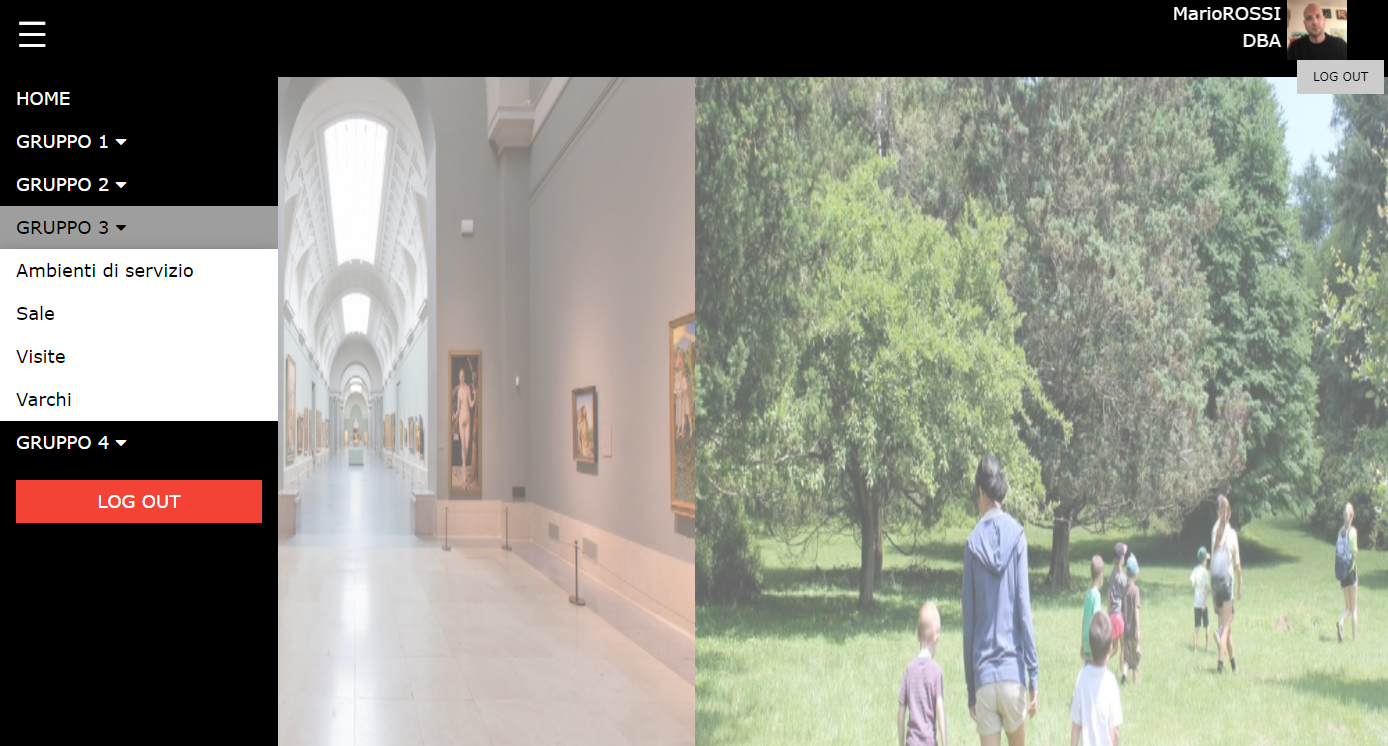
\includegraphics[scale=0.35]{Immagini/Header.png}
                \caption{Header visualizzato}                
            \end{figure}
            \begin{itemize}
                \item L'header deve essere presente in ogni pagina del sito Web
                \item L'header mostra in ogni pagina i il nickname e il ruolo dell'utente che ha effettuato il login
                \item L'header contiene un menu a tendina che è possibile aprire tramite il bottone in alto a sinistra
                \item Il menu a tendina contiene tutte le pagine web principali organizzate per gruppi 
            \end{itemize}
        \newpage
        \section{Form}
            \begin{figure}[httb]
                \centering
                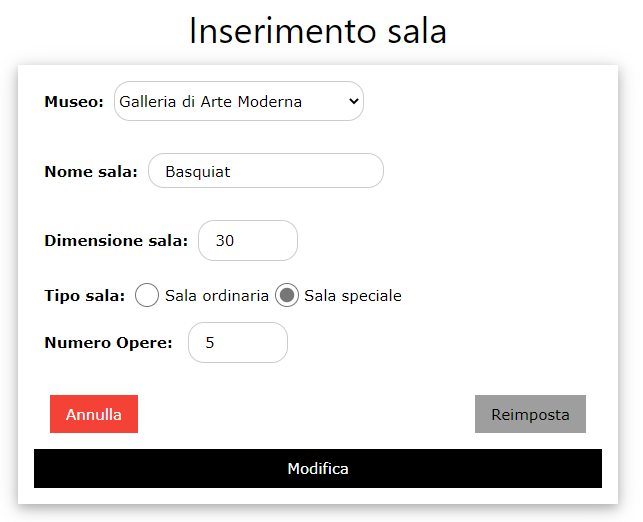
\includegraphics[scale=0.6]{Immagini/Form.png}
                \caption{Esempio di form}
            \end{figure}
            \begin{itemize}
                \item Utilizzare la procedura ApriForm e ChiudiForm per usare i Form.
                \item Per i campi di testo utilizzare InputText.
                \item Per i campi numerici utilizzare InputNumber.
                \item Per una lista di scelte utilizzare SelectOpen, SelectItem e SelectClose
                \item Per delle selezioni opzionali utilizzare InputCheckbox 
                \item Per delle selezioni obbligatorie utilizzare InputRadioButton
                \item Per ripristinare il form utilizzare InputReset
                \item Per inviare il risultato utilizzare InputSubmit
                \item Per annullare utilizzare un Collegamento ad una pagina scelta
            \end{itemize}
        \clearpage
        \section{Pagina di conferma}
            \begin{figure}[ht]
                \centering
                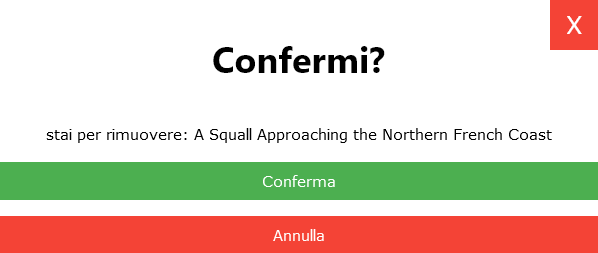
\includegraphics[scale=0.65]{Immagini/Conferma.png}
                \caption{Esempio di conferma}
            \end{figure}
            \begin{itemize}
                \item \textbf{Conferma:} Procede al controllo successivo e/o alla modifica del database.
                \item \textbf{Annulla:} Torna ad una pagina precedente senza ledere l'integrità del database.
            \end{itemize}
        \clearpage
        \section{Pagina di esito}
            \paragraph{}La procedura che mostra all'utente il risultato dell'operazione che ha effettuato è standard ed è presente
            all'interno del ModGUI.
            \begin{verbatim}
MODGUI1.REDIRECTESITO('Rimozione riuscita',
                    'Autore rimosso correttamente',
                    'Torna all'opera',
                    'Link opera',
                    'Parametri opera'
                    'Torna al menu'
                    'Link menu'
                    'Parametri menu');

MODGUI1.REDIRECTESITO('Rimozione fallita',
                    'Errore rimozione',
                    'Torna al menu',
                    'Link menu',
                    'Parametri menu');
            \end{verbatim}
            \begin{figure}[httb]
                \centering
                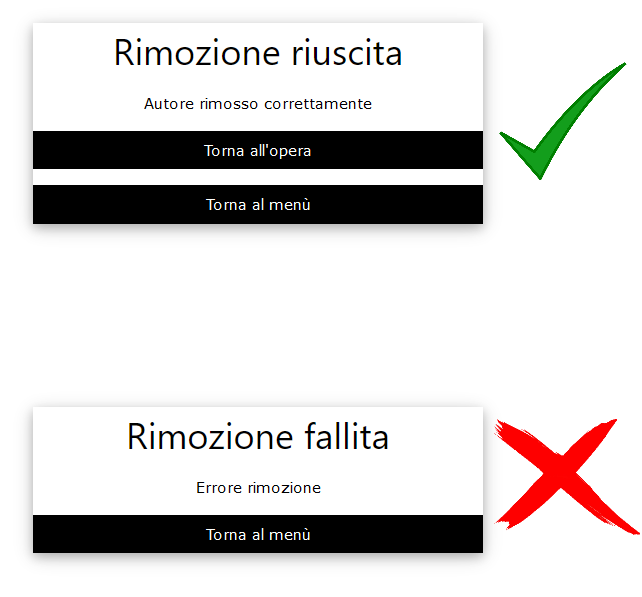
\includegraphics[scale=0.5]{Immagini/esitiOperazione.png}
                \caption{Esempi pagina di esito operazioni}
            \end{figure}
        \section{Diagramma filtraggio}
            \begin{figure}[ht]
                \centering
                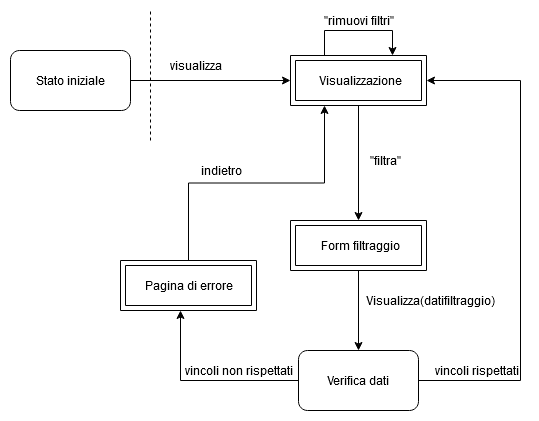
\includegraphics[scale=0.5]{Immagini/FiltraggioDiagramma.png}
                \caption{Diagramma filtraggio}
            \end{figure}
            \subsection{Visualizzazione}
                \paragraph{}La pagina viene visualizzata di default senza operazioni di filtraggio attive. Se vengono passati dei parametri la visualizzazione avviene
                secondo i criteri stabiliti.
            \subsection{Form filtraggio}
                \paragraph{}È il form in cui si stabiliscono le regole di filtraggio dei contenuti, può essere una barra di ricerca, un form di filtri o un ordinamento.
        \clearpage
        \section{Diagramma inserimento}
            \begin{figure}[httb]
                \centering
                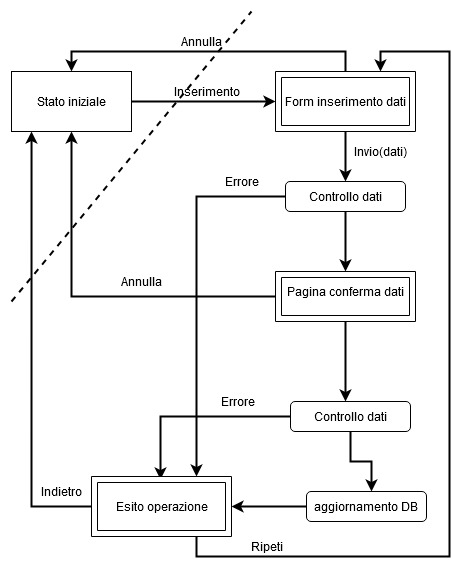
\includegraphics[scale=0.8]{Immagini/diagrammaInserimento.jpg}
                \caption{Diagramma inserimento}
            \end{figure}
            \subsection{Controllo dati}
                \paragraph{}I controllo verificano che i dati immessi rispettino i vincoli del database.
            \subsection{Pagina conferma dati} 
                \paragraph{}Pagina intermedia che permette all'utente di procedere o annullare l'inserimento.
            \subsection{Aggiornamento Database}
                \paragraph{}Il database viene aggiornato correttamente aggiungendo il record richiesto dall'utente.
        \section{Diagramma modifica}
            \begin{figure}[ht]
                \centering
                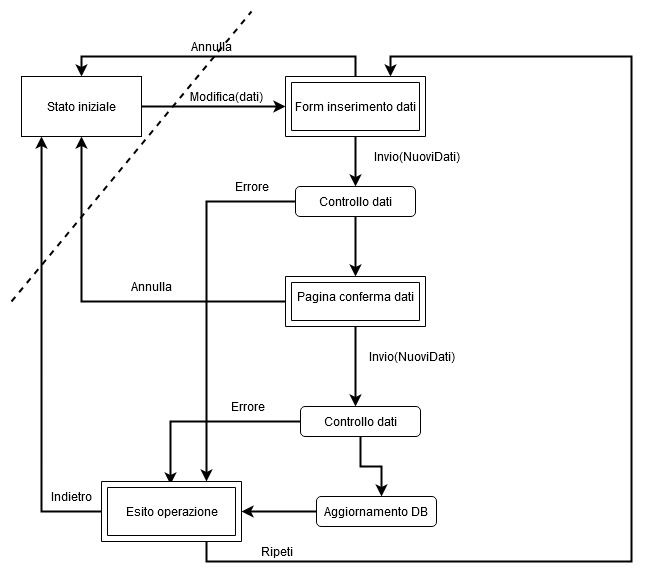
\includegraphics[scale=0.5]{Immagini/ModificaDiagramma.jpg}
                \caption{Diagramma modifica}
            \end{figure}
            \subsection{Form inserimento}
                \paragraph{}Nella modifica, a differenza dell'inserimento, nel form passiamo i parametri per precompilare i campi da modificare.
        \clearpage
        \section{Diagramma eliminazione}
            \begin{figure}[ht]
                \centering
                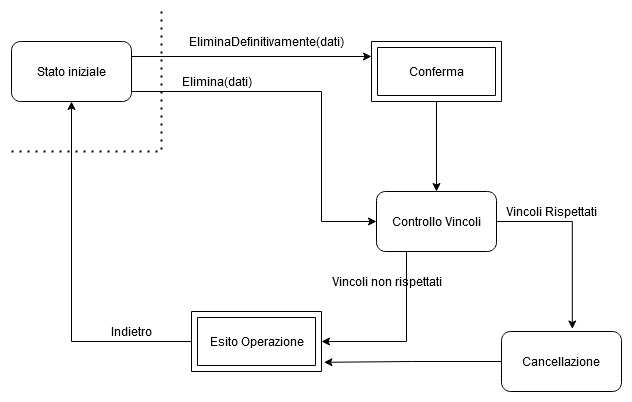
\includegraphics[scale=0.6]{Immagini/eliminazioneDiagramma.jpg}
                \caption{Diagramma eliminazione}
            \end{figure}
            \subsection{Conferma}
                \paragraph{}In caso di operazioni cruciali come le eliminazioni, è fortemente consigliato chiedere una conferma all'operatore.
            \subsection{Controllo vincoli}
                \paragraph{}Al fine di preservare l'integrità del database è necessario controllare, prima di eliminare definitivamente,
                le dipendenze con l'elemento e decidere il criterio di eliminazione.
            \subsection{Esito operazione}
                \paragraph{}Risultato dell'operazione, spiegato in dettaglio nella sezione precedente.
    \chapter{Autenticazione}
        \section{Accesso}
            \paragraph{}Il sistema, per visitare le pagine o interagire con le operazioni, richiede un accesso con delle credenziali.
            \textbf{La registrazione non è prevista}, gli utenti sono creati direttamente nel database dagli amministratori.\\
            È possibile accedere al form del login tramite il bottone in alto a destra \textbf{LOG IN}. 
            Il campo username dovrà essere composto da nome e cognome nel formato \textit{NomeCOGNOME} e la password dalla parola \textit{utente}.
            Il \textbf{LOG OUT}, o disconnessione, può essere effettuato tramite il bottone che apparirà passando sull'immagine dell'utente in alto a destra
            oppure con l'ultimo bottone del menu a tendina.
        \section{Sessioni}
            \paragraph{}Per \textbf{sessione} si intende una struttura dati che identifica l'utente che ha eseguito l'accesso per tutta la durata della sua permanenza.\\
            La sessione viene generata automaticamente quando l'utente accede correttamente e vengono registrati il suo \textbf{ID} e la \textbf{data e l'ora} di accesso.\\
            \textbf{Non può essere generata un'altra sessione sullo stesso utente se ne è gia presente una attiva.}
            Al termine della permanenza sul sito web, l'utente è invitato a effettuare il \textbf{LOG OUT} che \textbf{terminerà la sessione}
            aggiungendo la data e l'ora di disconnessione. 
        \section{Parametri}
            \paragraph{}Nessuna procedura deve ricevere come parametro idSessione poiché lo si raggiunge tramite i cookie e la funzione \textit{get\_id\_sessione}.
        \section{Funzioni}
            \begin{itemize}
                \item \textbf{hasRole(idSessione,'Ruolo'):} Questa funzione restituisce TRUE se il ruolo dell'utente che possiede come ID il primo parametro corrisponde con 'Ruolo'.
                \item \textbf{get\_id\_sessione:} Questa funzione restituisce l'ID dell'utente che ha effettuato il login.
            \end{itemize}
\end{document}